%% ------------------------------------------------------------
%% TITLE:     Vibrations and Waves - Summary of Three Types of Signal Oscillations
%% AUTHOR:    BINGHUAN W LI (Dept. Chemical Eng/Bio Eng, Imperial)
%% COMPILED:  XeLaTeX with TeX Live version 2023
%% LICENSE:   This work is licensed under a Creative Commons Attribution-NonCommercial 4.0 International License.
%% ------------------------------------------------------------

% Version History:
% v1.0  - xxxx-xx-xx - Initial draft
% v1.1  - 2024-11-06 - Reformatted the document

\documentclass[12pt,a4paper]{article}
\usepackage[margin=2cm]{geometry}
\usepackage{fontspec}
    \setmainfont{Times New Roman}
\usepackage{newtxmath}
\usepackage{amsmath, amsfonts, cancel}
\usepackage{enumitem}
\usepackage{float}

\usepackage{xcolor}
    \definecolor{linkcolour}{rgb}{0,0.2,0.6}
\usepackage[breakable]{tcolorbox}
% \usepackage{booktabs}
\usepackage{hyperref}
    \hypersetup{colorlinks,
                breaklinks,
                urlcolor=linkcolour,
                linkcolor=black,
                citecolor=black,
                pdftitle={Vibrations and Waves},
                pdfauthor={Li, Binghuan}}

            
\usepackage{tikz}
\usetikzlibrary{calc,patterns,decorations.pathmorphing,decorations.markings}
\usepackage[siunitx]{circuitikz}
\usetikzlibrary{arrows}

\usepackage{titling}
\setlength{\droptitle}{-4em}
\graphicspath{{./waves_images/}}
\setlength\parindent{0pt}
\linespread{1.15}

%=====================================================%
\begin{document}
\title{\textbf{Vibrations and Waves} \\ Transmission Lines}
\author{Binghuan Li\\ \href{mailto:binghuan.li19@imperial.ac.uk}{\texttt{binghuan.li19@imperial.ac.uk}}}
\date{\today}
\maketitle
%=====================================================%
\section{Motivation}
\begin{figure}[H]
    \centering
    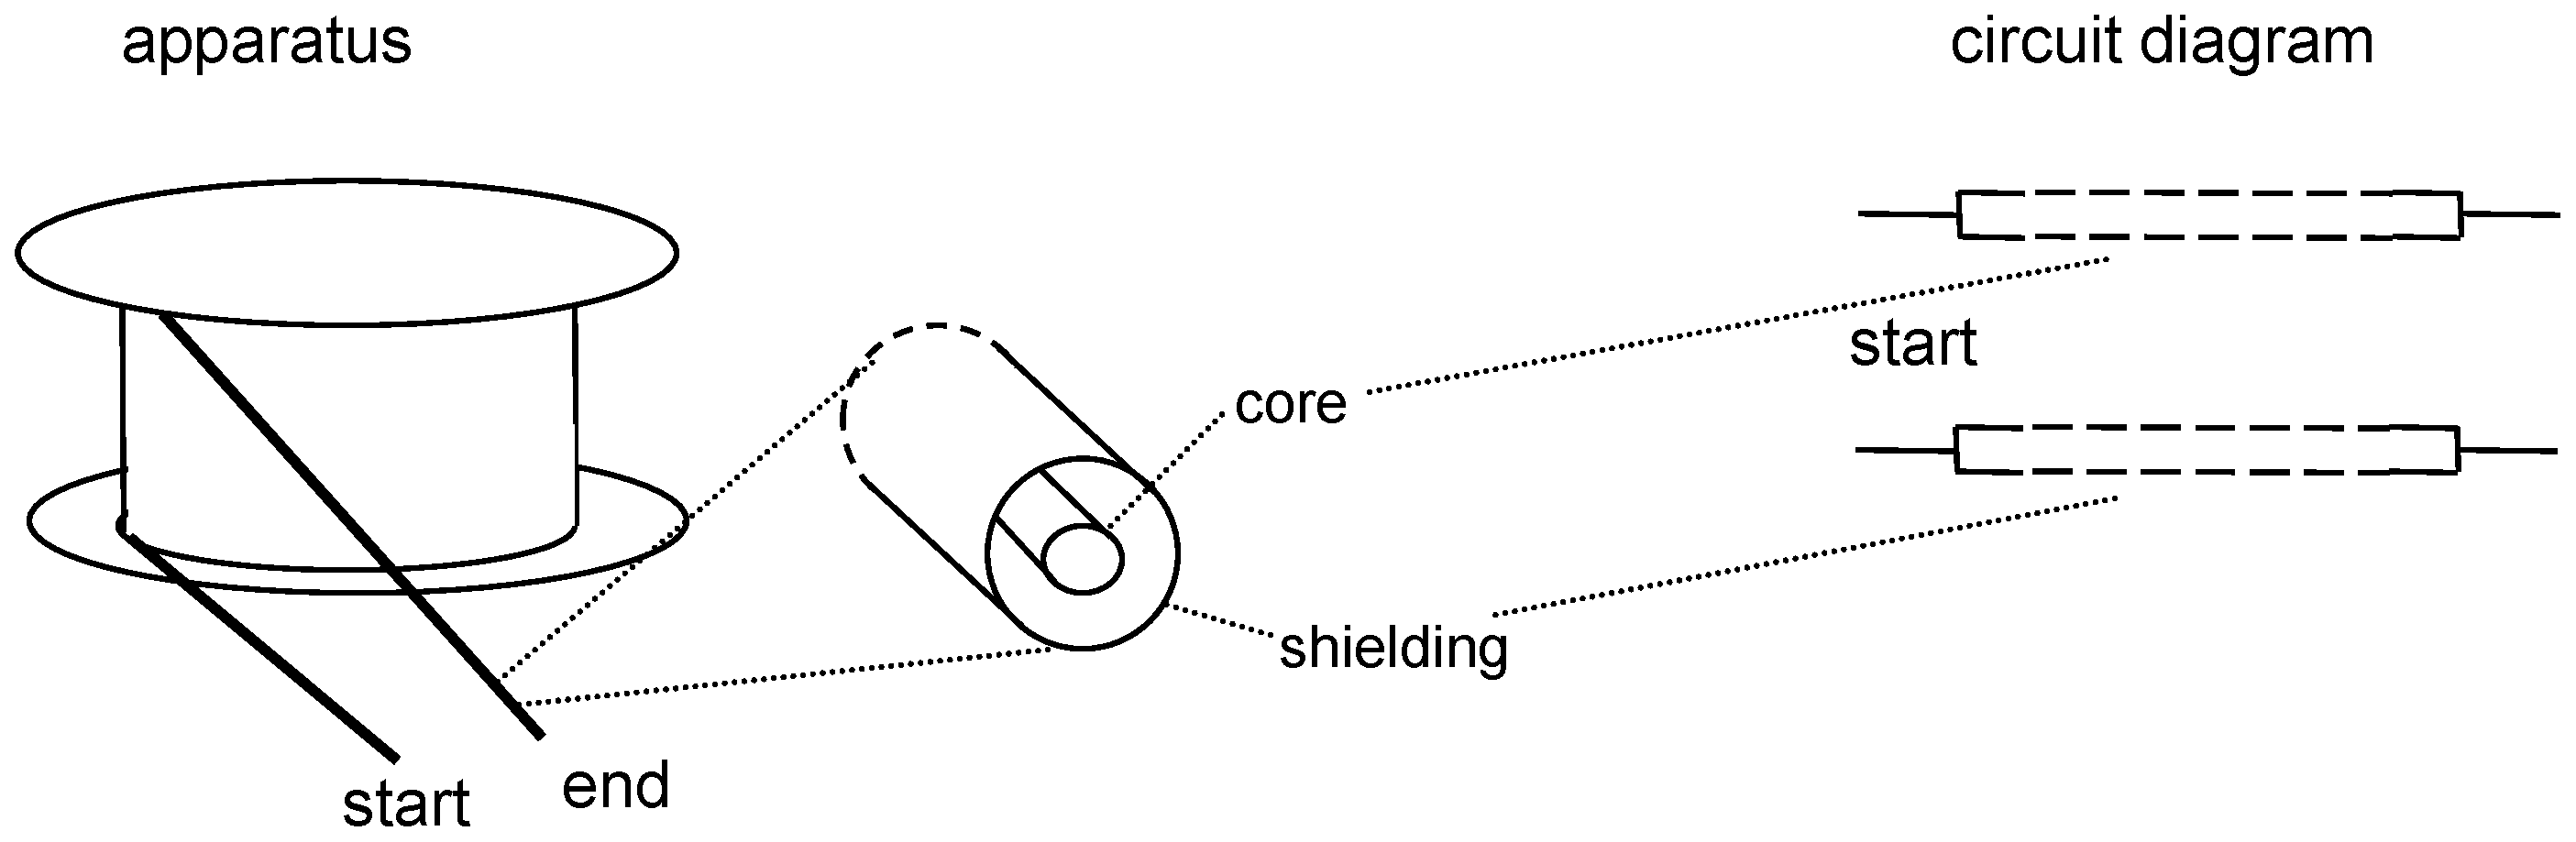
\includegraphics[width=.8\linewidth]{coaxial_cable.eps}
    \caption{Graphical illustration of the coaxial cable. Figure borrowed from the lab manual.}
    \label{fig:coaxial_cable}
\end{figure}
The transmission lines are ubiquitous in our real life, used to transmit signals. For example, a TV cable, shown in Figure \ref{fig:coaxial_cable}, which has a particular coaxial arrangement. Nevertheless, like the `traditional', or `normal' transmission lines we can imagine, they consist of two parallel conductors (or, the arrangement is equivalent to two parallel conductors!) - one proximal to the source (`start' in the figure), one distal to the source (`end' in the figure).

\begin{figure}[H]
    \centering
    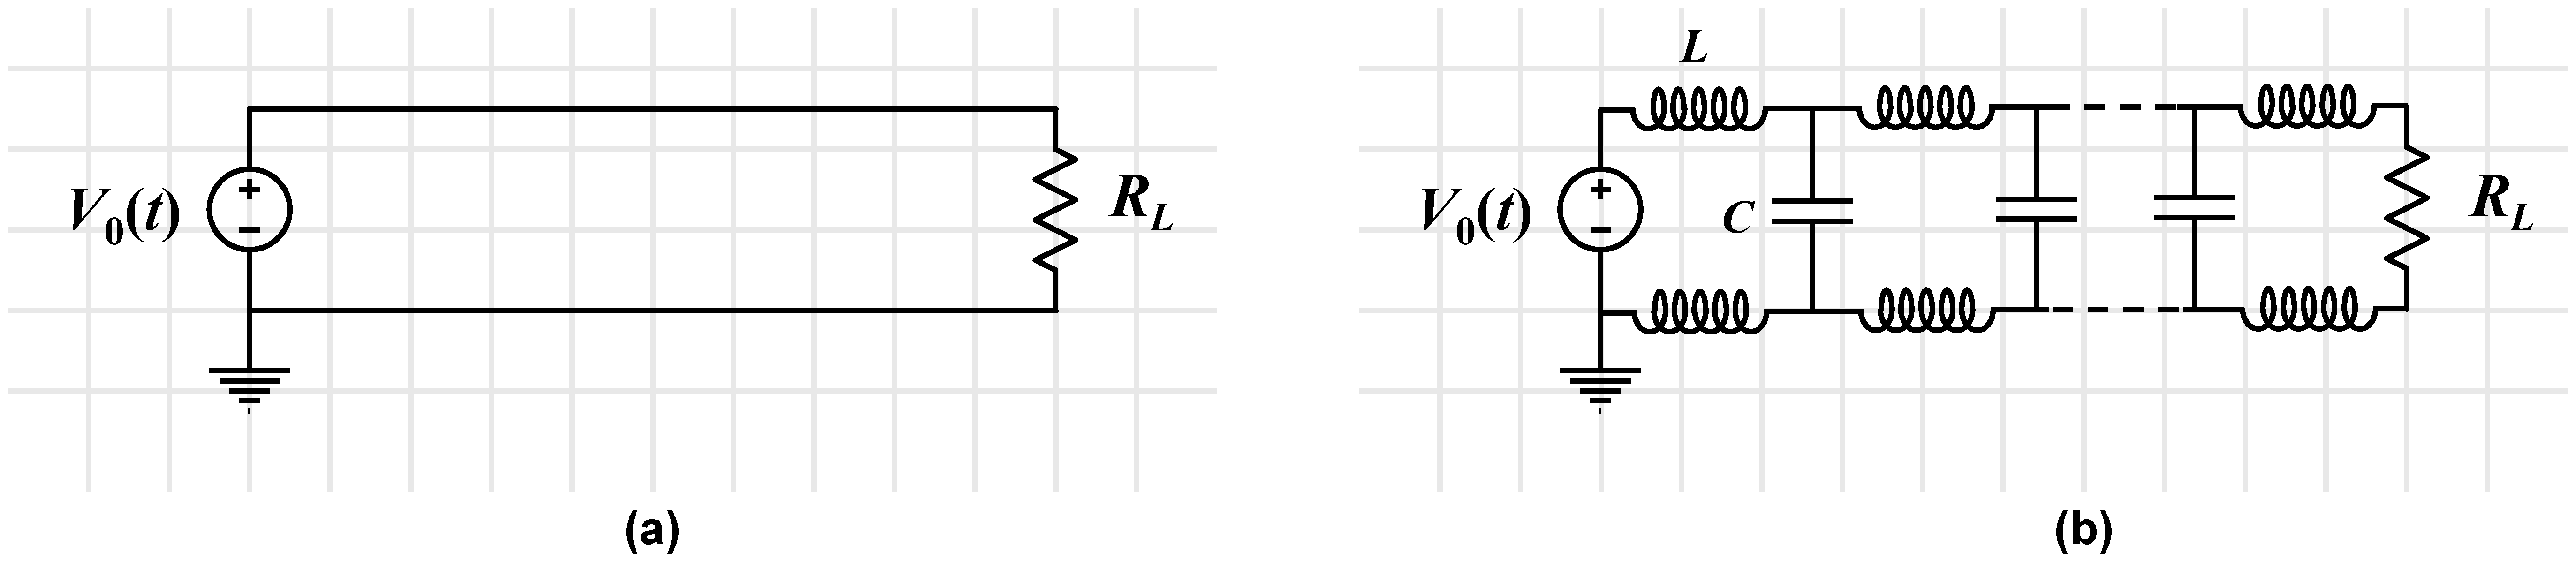
\includegraphics[width=\linewidth]{transmission_line.eps}
    \caption{(a) We previously assumed that any signal changes in $V_0(t)$ appears instantly on $R_L$. This is not true. (b) A more realistic model of electrical conduction needs to count the capacitative and inductive effects of the transmission lines.}
    \label{fig:transmission_line}
\end{figure}

Consider Figure \ref{fig:transmission_line}(a), previously, we assumed that any changes of $V_0(t)$ should appear \textit{instantly} on $R_L$. This is not true! Here are a few reasons to note:
\begin{itemize}
    \item The electrical signal is a wave that propagates at a speed around half of the light speed ($c \approx 3\times 10^8$ m/s). Hence, it takes time to travel to $R_L$.

    \item Electrical signal transmission relies on the transmission lines. All transmission lines have a capacitance relative to the ground and its neighbouring conductors.

    \item The transmission lines are self-inductive - due to their length.
\end{itemize}
Hence, a more realistic model is shown in Figure \ref{fig:transmission_line}(b). The behaviours of the signal transmitting in the transmission lines are predictable. Hence, the following sections shall exploit the signal behaviours by using simple mathematics, under both DC and AC excitations.
%=====================================================%
\section{Wave Propagation on a Transmission Line}
\subsection{Transmission Line Equations}
The first thing to note is the capacitance and inductance of any segment of a transmission line, as shown in Figure \ref{fig:transmission_line}(b), is proportional to the physical length of that segment. Therefore, to simplify our analysis, we consider the unit segment of the transmission line with the total length $\delta x$, as shown in Figure \ref{fig:unit_transmission_line}.

\begin{figure}[H]
    \centering
    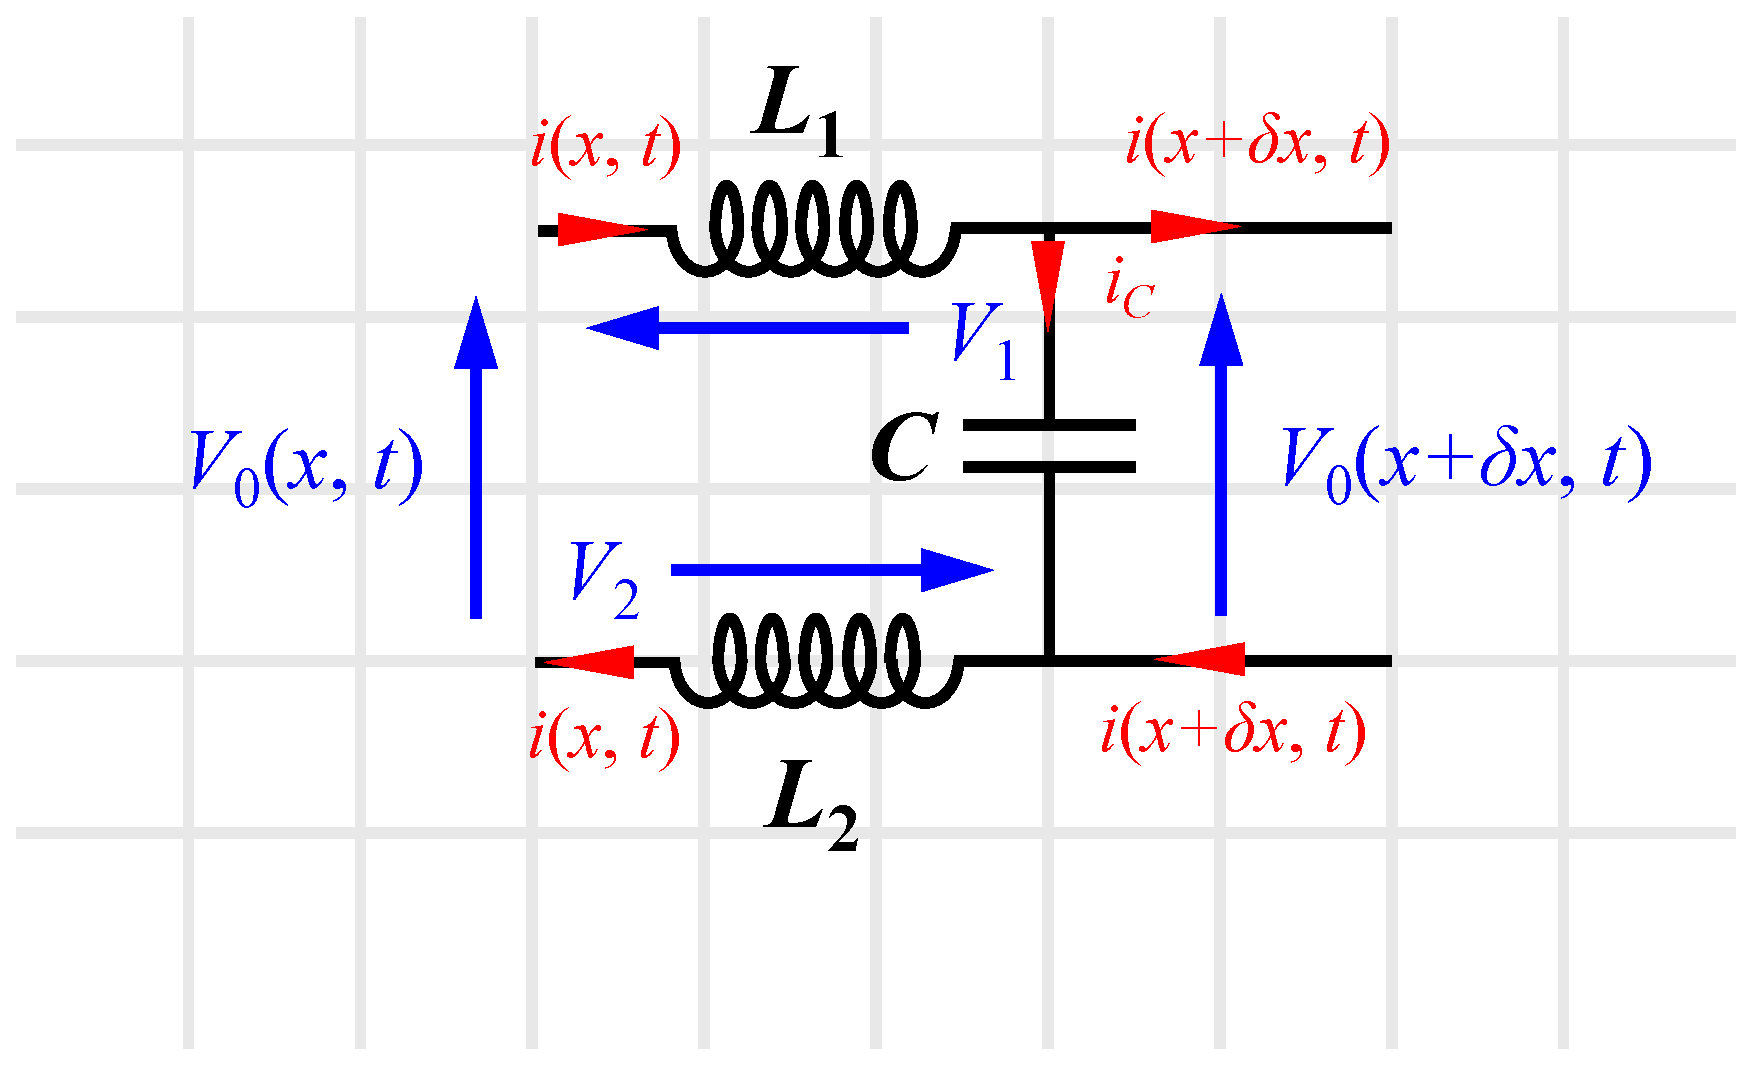
\includegraphics[width=0.6\linewidth]{unit_transmission_line.eps}
    \caption{Unit transmission line model with current and voltage annotations.}
    \label{fig:unit_transmission_line}
\end{figure}

Note that both the voltage and current here are time- and location-dependent, \textit{i.e.}, $V(x, t)$, $i(x, t)$.

\paragraph{Capacitative Equation}
By Kirchoff Current Law (KCL):
\begin{equation}
\label{eqn:KCL}
    i(x, t) = i_C + i(x+\delta x, t).
\end{equation}

With Equation \ref{eqn:KCL}, we rewrite $i_C = C \dfrac{\partial v}{\partial t}$, yielding
\begin{equation}
    i(x, t) = C \dfrac{\partial v}{\partial t} + i(x+\delta x, t)
    \quad \Rightarrow \quad
    C \dfrac{\partial v}{\partial t}  = i(x, t) - i(x+\delta x, t).
\end{equation}

Realizing $i(x+\delta x, t) - i(x, t) \equiv \dfrac{\partial i}{\partial x}$ (by definition of derivative!), the final form of the capacitive equation is
\begin{equation}
\label{eqn:capacitative}
\boxed{
    \frac{\partial i}{\partial x} = -C \frac{\partial v}{\partial t}.
}
\end{equation}
More commonly, we write $C \equiv C_0$, where $C_0$ is the capacitance \textit{per unit length}:
\[
    C_0 = C/\delta x \quad \quad {\color{gray} \rm [Farads/m]}
\]


\paragraph{Inductive Equation}    
By Kirchoff Voltage Law (KVL):
\begin{equation}
\label{eqn:KVL}
     V_0(x, t) = V_1 + V_0(x+\delta x, t) + V_2.
\end{equation}

Rewriting $V_1 = L_1 \dfrac{\partial i}{\partial t}$ and $V_2 = L_2 \dfrac{\partial i}{\partial t}$, plugging into Equation \ref{eqn:KVL}:
\begin{equation}
    (L_1 + L_2)\dfrac{\partial i}{\partial t} = V_0(x, t) - V_0(x+\delta x, t).
\end{equation}

Similarly, realizing $V_0(x+\delta x, t) - V_0(x, t) \equiv \dfrac{\partial v}{\partial x}$, resulting in final form of the inductive equation
\begin{equation}
\label{eqn:inductive}
\boxed{
     \frac{\partial v}{\partial x} = -(L_1+L_2) \frac{\partial i}{\partial t}.
}
\end{equation}
More commonly, we write $(L_1+L_2) \equiv L_0$, where $L_0$ is the inductance \textit{per unit length}:
\[
    L_0 = (L_1+L_2)/\delta x \quad \quad {\color{gray} \rm [Henries/m]}
\]

\paragraph{Combining Capacitative and Induction Equations}
Differentiating Equation \ref{eqn:inductive} by $x$, and differentiating Equation \ref{eqn:capacitative} by $t$
\begin{equation}
\label{eqn:inductive_dx}
    \frac{\partial^2 v}{\partial x^2} = -L_0 \frac{\partial^2 i}{\partial x \partial t},
\end{equation}
\begin{equation}
\label{eqn:capacitative_dt}
    \frac{\partial^2 i}{\partial x \partial t} = -C_0 \frac{\partial^2 v}{\partial t^2},
\end{equation}

Equating Equations \ref{eqn:inductive_dx} and \ref{eqn:capacitative_dt}, 
\begin{itemize}
    \item If we equate the voltage term, yielding
    \begin{equation}
    \label{eqn:transmission_line_eqn_vol}
    \boxed{
        \frac{\partial^2 v}{\partial x^2} = (L_0 C_0) \frac{\partial^2 v}{\partial t^2}
    },
    \end{equation}

    \item If we equate the current term, yielding
    \begin{equation}
    \label{eqn:transmission_line_eqn_curr}
    \boxed{
        \frac{\partial^2 i}{\partial x^2} = (L_0 C_0) \frac{\partial^2 i}{\partial t^2}
    }.
    \end{equation}
\end{itemize}

Equations \ref{eqn:transmission_line_eqn_vol} and \ref{eqn:transmission_line_eqn_curr} are known as the \textbf{transmission line equations}.

\subsection{Solution to Transmission Line Equations}
General solutions exist for Equations \ref{eqn:transmission_line_eqn_vol} and \ref{eqn:transmission_line_eqn_curr}, namely
\begin{align}
    v(x, t) & = f\left(t-\dfrac{x}{u}\right) + g\left(t+\dfrac{x}{u}\right) \\[1em]
    i(x, t) & = v(x, t) / Z_0
\end{align}
where $u$ is known as the \textbf{phase velocity}, $Z_0$ is known as the \textbf{characteristic impedance}. 

\paragraph{Phase Velocity} The phase velocity on a transmission line is given by
\[
    v = \frac{1}{\sqrt{L_0 C_0}}
\]

Define the angular frequency $\omega$, and the wave number $k = \dfrac{2\pi}{\lambda}$, the following relation satisfies
\[
    \omega = v k.
\]
A plot of $\omega$ versus $k$ is called a dispersion diagram. For an ideal transmission line, the dispersion diagram is a straight line.

\paragraph{Characteristic Impedance} The ratio of the instantaneous voltage to the instantaneous current for a single propagating disturbance on a transmission line is a constant called the characteristic impedance, 
\[
    Z_0 = \sqrt{\frac{L_0}{C_0}}.
\]

\subsection{Reflection and Transmission Coefficients}

Suppose a wave on a transmission line with the characteristic impedance $Z_0$ meets with a load with the impedance $Z_L$, the \textit{reflected} wave is generated. \\

The voltage across the load is the sum of the incident voltage and the reflected voltage:

\[
    V_L = V_r + V_i.
\]

The current in the load is the sum of the incident current and the reflected current:
\[
    i_L = i_r + i_i
\]

By Ohm's law:
\[
    i_i = \frac{V_i}{Z_0} 
    \quad \quad
    i_r = \frac{V_r}{Z_0}
    \quad \quad
    i_L = \frac{V_L}{Z_L}
\]
This allows us to derive the 
\[
    K_v = \frac{V_r}{V_i} = \frac{Z_L - Z_0}{Z_L + Z_0}
    \quad \quad
    K_i = \frac{i_r}{i_i} = \frac{Z_0 - Z_L}{Z_L + Z_0}
    \quad \quad
    T_v = \frac{V_L}{V_i} = \frac{2Z_L}{Z_L + Z_0}
    \quad \quad
    T_i = \frac{i_L}{i_i} = \frac{2Z_0}{Z_L + Z_0}
\]
where $K_v$ is the voltage reflection coefficient, $K_i$ is the current reflection coefficient, $T_v$ is the voltage transmission coefficient, and $T_i$ is the current transmission coefficient.

%=====================================================%
\section{DC Signals on a Transmission Line}
When the switch closes, the incident wave carries a voltage, $v_i$, and propagates to the load.
\[
    v_i = \frac{Z_0}{Z_0+R} V_0
\]

After the wavefront reaches the load, the wave is reflected, with the voltage $v_r$ being 
\[
    v_r = \frac{Z_L-Z_0}{Z_L+Z_0} v_i.
\]

After the reflected wave reaches the source (\textit{i.e.}, the beginning), it is reflected to the load again. Note that the $R$ now is seen as the `load resistance`, hence the reflection coefficient is $\dfrac{R-Z_0}{Z_0+R}$. The reflected voltage $v''_r$ is
\[
    v'_r = \frac{R-Z_0}{Z_0+R} v_r 
\]
Again, the wave is reflected for the 3\textsuperscript{rd} time after reaching the load, being
\[
    v''_r = \frac{Z_L-Z_0}{Z_L+Z_0} v'_r.
\]
And so on. \\

What is the voltage that appears on the load $R_L$, eventually? We can simply summing the incident voltage $v_i$, and all reflected voltage $v_r$, $v'_r$, $v''_r$, ..., resulting
\begin{align}
\begin{split}
    v_L 
    &= v_i + \frac{Z_L-Z_0}{Z_L+Z_0} v_i + \frac{R-Z_0}{Z_0+R} v_r + \frac{Z_L-Z_0}{Z_L+Z_0} v'_r + ... \\
    &= v_i + \frac{Z_L-Z_0}{Z_L+Z_0} v_i + \frac{R-Z_0}{Z_0+R}\frac{Z_L-Z_0}{Z_L+Z_0} v_i + \frac{R-Z_0}{Z_0+R} \left(\frac{Z_L-Z_0}{Z_L+Z_0}\right)^2 v_i + ...
\end{split}
\end{align}

Denote $\frac{Z_L-Z_0}{Z_L+Z_0} = K_{vL}$ and $\frac{R-Z_0}{Z_0+R} = K_{vS}$, we see a more concise expression of $v_L$, as 
\begin{equation}
    v_L = v_i + K_{vL} v_i + K_{vL}K_{vS} v_i + K_{vL}^2 K_{vS} v_i + ...
\end{equation}
which is the summation of two geometric sequences, $v_L = S_1 + S_2$
\begin{align}
    (\text{sequence 1}) &\quad
    S_1 = v_i (1 + K_{vL} K_{vS} + K_{vL}^2 K_{vS}^2 + K_{vL}^3 K_{vS}^3 + ...) = \frac{v_i}{1-K_{vL}K_{vS}} \ ,\\
    (\text{sequence 2}) &\quad
    S_2 = v_i  K_{vL} (1 + K_{vL} K_{vS} +  K_{vL}^2 K_{vS}^2 + K_{vL}^3 K_{vS}^3 + ...) = \frac{v_i  K_{vL}}{1-K_{vL}K_{vS}} .
\end{align}
Therefore,
\begin{equation}
    v_L = \frac{v_i}{1-K_{vL}K_{vS}} + \frac{v_i K_{vL}}{1-K_{vL}K_{vS}} = v_i \frac{Z_L (R+Z_0)}{Z_0 (R+Z_L)}.
\end{equation}
Since $v_i = \dfrac{Z_0}{R+Z_L} V_0$,
\begin{equation}
    v_L = \frac{Z_L}{R+Z_L} V_0,
\end{equation}
which is of expected.
%=====================================================%
\section{AC Signals on a Transmission Line}
\subsection{AC Excitation}
The voltage at the incident end of the line 
\[
    v_i (0) = \frac{Z_0}{Z_0 + R} \quad \text{for} \quad V = V_0 e^{j \omega t}
\]
The voltage at a point with a distance $\ell$ from the origin
\[
    v_i (\ell) = \frac{Z_0}{Z_0 + R} \quad \text{for} \quad V = V_0 e^{j (\omega t-k \ell)}
\]

or, in the negative direction:
\[
    V = V_0 e^{j (\omega t+k \ell)}
\]

\subsection{Impedance Transformation}
For all the waves travelling towards the load, the summation of the voltage and current are
\begin{align*}
    v_{+} & =  V_{+} e^{j (\omega t - kx)} \\
    i_{+} & = \frac{V_{+}}{Z_0} e^{j (\omega t - kx)} \ .
\end{align*}
Similarly, for all the waves travelling backwards to the source:
\begin{align*}
    v_{-} & =  V_{-} e^{j (\omega t + kx)} \\
    i_{-} & = -\frac{V_{-}}{Z_0} e^{j (\omega t + kx)} \ .
\end{align*}
\paragraph{At the Load End}
The voltage and current seen on the load ($x=0$) is
\begin{align*}
    v_L & = v_{+}(x=0) + v_{-}(x=0) \\
    i_L & = i_{+} - i_{-} = [v_{+}(x=0)-v_{-}(x=0)]/Z_0 \,
\end{align*}
Since the impedance of the load is $ Z_L = \dfrac{V_L}{i_L}$, we can therefore depicts the relation between $v_{+}(x=0)$ and $v_{-}(x=0)$ as
\[
    \dfrac{v_{-} (x=0)}{v_{+} (x=0)} = \frac{V_{-} \cancel{e^{j (\omega t)}}}{V_{+} \cancel{e^{j (\omega t)}}} = \frac{\text{indident wave}}{\text{reflected wave}} = \frac{Z_L - Z_0}{Z_L + Z_0} = K_v.
\]

\paragraph{At the Source End}
The voltage and current seen on the source end ($x=-\ell$) is
\begin{align*}
    v_s & = v_{+}(x=-\ell) + v_{-}(x=-\ell) = V_+ e^{j(\omega t+ k\ell)} + V_{-}e^{j(\omega t-k \ell)} \\
    i_s & = i_{+} - i_{-} = [v_{+}(x=0)-v_{-}(x=0)]/Z_0 = \frac{V_{+}}{Z_0} e^{j\omega t} (e^{jk\ell} - K_v e^{-jk\ell}) \,
\end{align*}


\[
\boxed{
    Z_{\rm in} = Z_0 \frac{Z_L + j Z_0 \tan k \ell}{Z_0 + j Z_L \tan k \ell}
}
\]



\begin{itemize}
    \item If $Z_L = 0$: short circuit on the end of the line. $Z_{\rm in} = Z_0 \tan k \ell$, where $k = 2 \pi / \lambda$, we can conclude that $Z_{\rm in}$ is length dependent, measured in wavelength. Consider:
    
    \begin{itemize}
        \item For $\ell \ll \lambda$, then $k \ell \ll 1$, by small angle approximation, $\tan k \ell \approx k \ell$, $Z_{\rm in} \approx 0$.

        \item As $\ell$ increases but $k \ell < 1$, $Z_{\rm in} = j Z_0 k \ell$

        \item For $\ell = \dfrac{\lambda}{4}$, $k \ell = \pi/2$, $Z_{\rm in} \approx j Z_0 k \ell$

        \item For $\lambda/4 < \ell < \lambda/2$, $\tan k\ell < 0$,
    \end{itemize}

    \item If $Z_L = \infty$, an open circuit at the end of the line. $Z_{\rm in} = \dfrac{-j Z_0}{\tan k \ell}$. Consider:
    \begin{itemize}
        \item For $k \ell \ll 1$, $Z_{\rm in} \to \infty$.

        \item For $\ell = \lambda /8$, $Z_{\rm in} = -j Z_0$.

        \item For $\lambda/4 < \ell < \lambda/2$, $Z_{\rm in} = j$.
    \end{itemize}
    
\end{itemize}

\end{document}